\documentclass{llncs}
%\documentclass[a4paper]{article}

\usepackage{fullpage}
\usepackage{setspace}
\usepackage{url}
\usepackage{algorithmic}
\usepackage{algorithm}
\usepackage{amsmath}
\usepackage{latexsym}

\usepackage{graphicx}
\usepackage{subfig}

\onehalfspacing

%\newtheorem{definition}{Definition}
%\newtheorem{theorem}{Theorem}
%\newtheorem{example}{Example}
\newtheorem{query}{Query}

%\newcommand{\nop}[1]{}

\title{Mapping Microblog Posts to Encyclopedia Articles}
\author{Uta L\"{o}sch \and David M\"{u}ller \and Andreas Harth}
\institute{
	Karlsruhe Institute of Technology (KIT), D-76131 Karlsruhe, Germany\\ 
	\email{uta.loesch@kit.edu},\\
	\email{david.mueller@student.kit.edu},\\
	\email{harth@kit.edu}
}
\begin{document}

\maketitle

\begin{abstract}
Search results on Twitter are hard to analyze and read. To facilitate understanding the meaning of a search term in the context of Twitter, we have developed a system which annotates search results with entities that best describe the search result, thus offering a means of quickly grasping the meaning of the search results and at the same time providing starting points for further exploration of the search results' context. In an evaluation we show that the entities used for annotation represent the tweet's content in a suitable manner and that the annotations remain stable over time, i.e. when executing the same search at different times, the same entities are returned.
\end{abstract}

Keywords: Twitter, Wikipedia, DBpedia, RDF

\section{Introduction}

Twitter\footnote{\url{http://twitter.com}} is a micro-blogging service that has become very influential over the last years. The idea of micro-blogs is the same as that of blogs, except that the message length is restricted to 140 characters. Twitter has a total of about 190 million of users who produce 65 million twitter messages a day. Thus, twitter represents a huge data source on the web.

Twitter offers the possibility to search for twitter messages containing a specific term or hash tags. This search returns a fixed number of most recent messages containing the search term. However, it is hard to grasp the context of the results and to get further information on the topic that was searched for. As each single twitter message is very short and contains little information, it is necessary to parse the whole set in order to get an overview of the context(s) in which the search term is used. To facilitate this putting into context of the search results, we propose to annotate search results with a set of entities which reflect the content of the result feeds. These entities will not only help to understand the search terms, but also serve as a starting point for refining the search or searching for further information related to the search result. 

On twitter, hash tags are frequently used to associate messages with a specific topic, place, person or evecnt. For example, twitter messages talking about what is going on at the European Semantic Web Conference 2011 will probably be tagged with $\#eswc2011$. If a user encounters this hash tag and does not understand it, he can search for this hash tag. Using our approach the search will not only return messages using the tag but also a set of entities which have been detected in the search result. These tags will help the user to gain an understanding in which context the hash tag is used and what it may mean.
% Konzept von Hashtags genauer erkl�ren? Warum sind Hashtags sinnvoll?
In this paper, we present a system which automatically annotates a Twitter search result with Wikipedia entities. While it would be more interesting to annotate each single twitter message with relevant entities, twitter messages are too short to contain much relevant information which could be used as input for the annotation tool. Thus, we chose to generate annotations for the whole search result. 

The motivation for choosing Wikipedia entities was that it offers a wide coverage of topics. Furthermore, automatic tools for annotating text with Wikipedia entities are readily available (see \cite{key:wikifier}).

Annotations should be stable over time, unless the topics discussed in the twitter messages containing the search term change. In an evaluation of our approach we have tried to analyze the stability of the result.

Our contributions thus are:
\begin{itemize}
	\item an approach for finding entities which are related to a search on twitter
	\item an implementation of our approach
	\item an evaluation of the stability and relevance of the entities found with our approach.
\end{itemize}

The rest of this paper is organized as follows: in Section~\ref{sect:relWork} we discuss related work, in Section~\ref{sect:method} we present our approach, the results of our evaluation are presented in Section~\ref{sect:eval}, before we conclude in Section~\ref{sect:conclusion}.

\section{Related Work}
\label{sect:relWork}

Bringing Semantic Web technologies and Semantic Web technologies together, has been proposed before: Passant et al. \cite{key:smob} have proposed a data model for making twitter data available on the Semantic Web. They propose a data model which allows for the association of URIs with users, microblogs and microposts. To this end, SIOC and FOAF vocabularies are used and extended. Specifically, the new concepts \emph{Microblog} and {MicroBlogPost} are introduced. Additionally, they propose the use of so-called semantic hash tags. The idea is to use URIs as hash tags (e.g. \emph{\#geo:Paris\_France}). It becomes thus possible to link microposts to entities in the Linked Open Data cloud.

A system for mapping text to Wikipedia entities has been proposed by Milne and Witten \cite{key:wikifier}. 
%System beschreiben



\section{Method Overview}
\label{sect:method}

The implemented
system\footnote{\url{http://km.aifb.kit.edu/services/twittersearchwrap/}} (further called Twitter Search Wrapper) is called with a query representing
the twitter search term and returns a RDF\footnote{\url{http://www.w3.org/RDF/}}
document semantically describing the most recent twitter posts matching the
given query. The returned RDF document furthermore contains a mapping of the
query to Encyclopedia articles which based on the content published by users that most recently used the search
term in their posts maps to articles best describing the content of Twitter
messages related to the term. An overview of the System Architecture is given in Figure
\ref{fig:arch}.\newline Taking a more detailed look, methods performed by the
Twitter Search Wrapper can be grouped into five sequential steps (see Figure
\ref{fig:arch}). We will follow those steps along a simple example, using
\#ka (a hashtag frequently used to describe posts related to the city of
Karlsruhe, Germany) as search term for the Twitter Search wrapper.

 
\begin{figure}[htb]
  \centering
  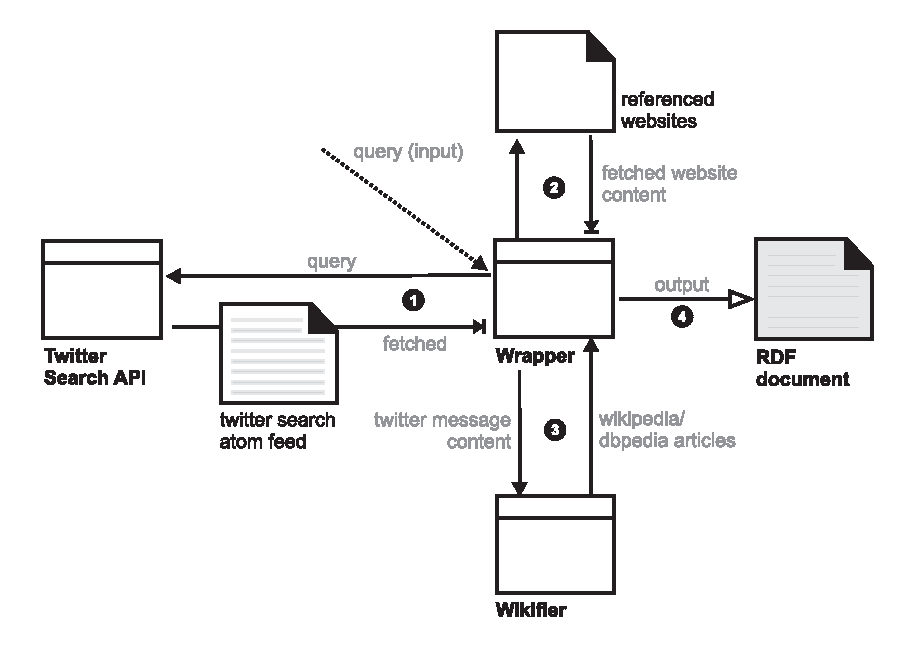
\includegraphics[width=.6\linewidth]{architecture}
  \caption{System Architecture}
  \label{fig:arch}
\end{figure}

% 1. Schicke Suchanfrage an Twitter Search API
% Ich w�rde etwas ausf�hrlicher erkl�ren, was die Twitter Search API macht (an welcher Stelle im Paper m�sste man nochmal �berlegen).
% 2. Greife Ergebnisse ab

\begin{enumerate}
  \item 
In a first step the Twitter Search Wrapper fetches the atom feed (XML Data)
generated by the Twitter Search
API\footnote{\url{http://dev.twitter.com/doc/get/search}} for a given
search query. The generated feed contains the data of the 100 most recently published
publicly visible Twitter messages and their authors which match the search query.
The messages themselves are described by their content, publishing date, authors
and optionally a geographic location.\linebreak\linebreak
In the given example, calling the Wrapper with query '\#ka' will return a
document containing all most recent Twitter posts and their meta information
whose content matched the search string '\#ka'. Taking a closer look, a single
retrieved post might have the following content: \newline\linebreak 
\texttt{Just returned from a wonderful holiday in \#ka.
\url{http://www.karlsruhe.de/stadt/tourismus.en} @KarlsruheTweets}
\linebreak
\item
In a second (optional) step hyperlinks posted in messages of the fetched
feed are followed, content of the referenced website's body is fetched and
processed to the Wrapper. This option is triggered calling the Twitter Search
Wrapper with attribute extern=true.\newline
\linebreak
Following the initial example, the given sample post contained a link to
\url{http://www.karlsruhe.de/stadt/tourismus.en}, the official homepage of the tourist office of the city of Karlsruhe, which contains the following
text:\newline
\linebreak
''\texttt{Karlsruhe, where paths converge - a legendary city in the sunny
south-west of Germany,\newline famed for its fan-shaped historic street plan,
where margraves reigned in times past,\newline and German joie de vivre reigns
today.}''\newline\linebreak
The text is fetched and returned to the Wrapper. The same accounts for
content of all other websites that were referenced in the list of posts matching
the query \#ka.\newline
\item
The Wrapper now calls the Wikifier (see \cite{key:wikifier}). Content of
the Twitter messages that matched the search query and optional content of their
referenced websites is merged to a single input string which is used as input for the Wikifier. The service
returns a list of matching articles of the English
Wikipedia. Optionally the wrapper can be initially called with attribute lang=de
to trigger mapping to the German Wikipedia.\newline\linebreak
In the given example, content of all posts related to the search term '\#ka' is
merged with retrieved external website content. Taking a closer look at the
single post we merge its content and content of its referenced website to
a single string:\newline\linebreak
\texttt{Just returned from a wonderful holiday in \#ka.
\url{http://www.karlsruhe.de/stadt/tourismus.en} @KarlsruheTweets. Karlsruhe,
where paths converge - a legendary city in the sunny\newline south-west of
Germany, famed for its fan-shaped historic street plan, where margraves\newline
reigned in times past, and German joie de vivre reigns today.}\newline\linebreak
This string is appended to Twitter content and external content of all other
posts that have been retrieved in this way matching the initial query \#ka and
used as input for the Wikifier.\newline
  \item
The Wikifier now maps the input string to relevant Wikipedia articles. A
detailed description of this process can be found under \cite{key:wikifier}. 
The list of matching Wikipedia articles is finally returned to the
Wrapper.\newline\linebreak
In the given example, a desired mapping of the contents of posts related to the
hashtag \#ka and mapping for the hashtag \#ka as such, would preferably be a
mapping to Wikipedia articles describing content related to Karlsruhe. We just
assume this results in mappings to the articles for Karlsruhe, Germany and the
Karlsruhe\_Institute\_of\_Technology.\newline
  \item
The Wrapper finally generates a RDF document using popular ontologies
(foaf\footnote{http://xmlns.com/foaf/spec/},
dublincore\footnote{http://dublincore.org/documents/dcmi-terms/}, geo\footnote{http://www.w3.org/2003/01/geo}) to describe the data related to the
returned Twitter messages and their content using 'rdfs:seeAlso' triples to link
the document to DBPedia\footnote{\url{http://dbpedia.org/About}} URIs (converted
output of the Wikifier) that have been mapped to the documents content.
At this point DBPedia is chosen as referenced encyclopedia, because its
semantic nature and description of Wikipedia article content contributes to a
coherent semantic description. \newline\linebreak Coming back to the example,
the output RDF document containes the following triples to reference the DBPedia
mappings:\newline\linebreak \texttt{<rdfs:seeAlso
rdf:resource="http://dbpedia.org/resource/Karlsruhe"/>}\newline
\texttt{<rdfs:seeAlso
rdf:resource="http://dbpedia.org/resource/Germany"/>}\newline
\texttt{<rdfs:seeAlso rdf:resource="http://dbpedia.org/resource/\newline
Karlsruhe\_Institute\_of\_Technology"/>}\newline\linebreak 
The twitter posts matching the search term \#ka are all described in the output
document. As an example, the description for the initially given post might
result in the following RDF output:\newline\linebreak
\texttt{<rdf:Description
rdf:about="http://km.aifb.kit.edu/services/twitterwrap/statuses/\newline
show/1234567890\#id">\newline <foaf:page
rdf:resource="http://twitter.com/sample\_user\_12345/statuses/1234567890"/>\newline
<dc:date>2011-02-23T12:00:00Z</dc:date>\newline
<geo:lat>49.010239</geo:lat>\newline <geo:long>8.411879</geo:long>\newline
<foaf:maker
rdf:resource="http://km.aifb.kit.edu/services/twitterwrap/users/\newline
show?screen\_name=sample\_user\_12345\#id"/>\newline <dc:description>\newline
Just returned from a wonderful holiday in \#ka.
\url{http://www.karlsruhe.de/stadt/tourismus.en} @KarlsruheTweets\newline
</dc:description>\newline
</rdf:Description>\newline}
\end{enumerate}

\section{Experiments and Evaluation}
\label{sect:eval}

Trending topics are listed in Table \ref{tbl:terms}.

\begin{table}[ht*]
\centering
\begin{tabular}{ c }
Search term                    \\
\hline
\#s21 \\
Karlsruhe\\
\end{tabular}
\caption{Search terms}\label{tbl:terms}
\end{table}

\begin{definition}[Stability]

\end{definition}


\section{Conclusion}
\label{sect:conclusion}




\bibliographystyle{abbrv}
\bibliography{bib}

\end{document}
